\subsection{Project Overview}
Our project is a proof of concept to determine the usability of the NVIDIA Jetson TX1 for aerospace computer vision applications.  It demonstrates this capability by processing multiple video streams with multiple image filters at high frame rates and low latency. This program is designed to run without needing any interaction from the user, however we have included the ability to switch between different video processing modes in order to demonstrate the various filters and camera views.
\par
The HawkEye Vision System captures video from cameras, processes it using various filter algorithms, and displays it on the screen. It utilizes both the CPU and GPU simultaneously to create a very high throughput, low latency video feed. The CPU portion of the program is responsible for capturing video from the camera using Point Grey's Flycapture API, and managing the parameters of the GPU programs (which are called kernels). The CPU program also manages user input and sets up the OpenGL output system. 

\begin{figure}[H] 
	\centering
	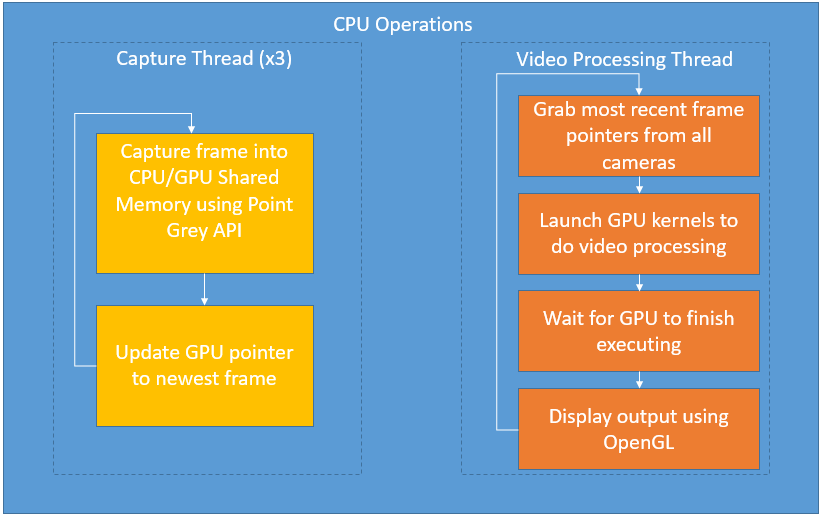
\includegraphics[width=0.6\textwidth,natwidth=610,natheight=642]{images/CPU.png} 
	\caption{CPU Operation - showing the functions of the different CPU threads}  
	\end{figure}
	
The GPU does all the heavy lifting in this program. It performs multiple video processing operations simultaneously. The GPU program is divided into several streams, each of which operates independently of the others, much like the multiple threads on a CPU. The Jetson allows multiple GPU kernels to run at the same time, as long as they are in different streams.
In the following diagram, each box represents a different GPU Kernel (with the exception of the bottom right box which is actually the same as the three bottom left kernels, just abbreviated to save space). These kernels are executed in order by their corresponding CUDA streams, which is essential. 
	
\begin{figure}[H] 
	\centering
	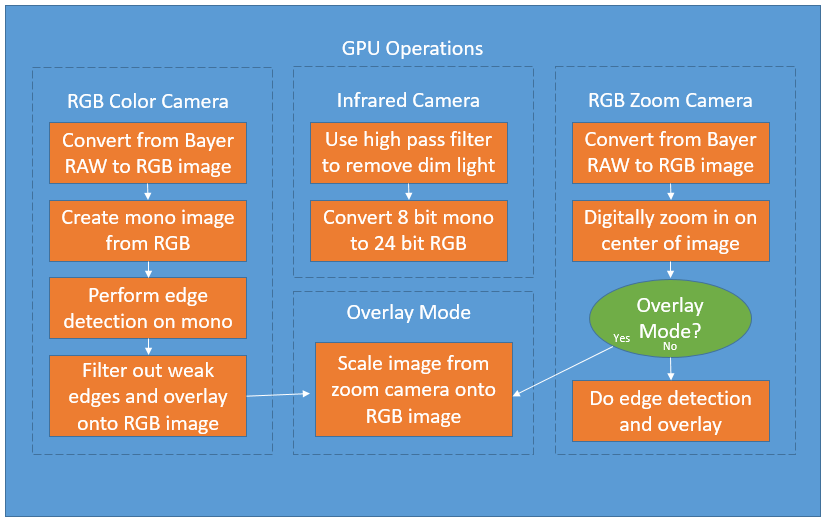
\includegraphics[width=0.6\textwidth,natwidth=610,natheight=642]{images/GPU.png}
	\caption{GPU Operation - showing the functions of the different CUDA streams}  
	\end{figure}
	
\subsection{Project Results}
Our project defines specific latency, frame rate, and resolution requirements in order for our system to be a viable option to replace the current FPGA system. Our end-to-end latency requirement specifies that it should take less than 100ms to capture video from the camera, process it, and display the output stream. Additionally, we are required to process a minimum of 30 frames per second at 1080p resolution. Our goal is to perform as much image processing as we can while maintaining these performance metrics.
\par
In order to measure the latency of our application, our software contains a detailed, built-in performance logging system. Each component of the software is separated into polymorphic, class-based, HawkEye modules. Each individual module measures execution time including the time it takes to transfer the results to the next module. The overall latency for each frame is determined by the time it takes for all modules to finish executing from input to output, counted as the sum of the longest path. It is important to measure each individual module's latency as well as the overall latency because not all cameras are going to be subjected to the same filtering algorithms. The additional information will enable us to predict the outcome latency based on the set of modules used. In order to measure the frame rate, we simply count the number of frames processed in a second.
\par
Our goal is to support independent image processing of three separate inputs. Rockwell Collins has given us some challenges outside of our requirements, which we will try to implement. We have multiple types of cameras with different lenses: two standard RGB cameras and one NIR (Near infrared) camera. The IR camera will be used to identify high intensity point lights, which we will then overlay onto the processed input from one of the RGB cameras. In the industry, this would be used to identify runway lights for landing aircraft. The third camera would provide a more focused look at the target. The first performance benchmark we need to determine is to simply get three simultaneous camera feeds running at the full 30 frame per second.\\

\begin{figure}[H]
\centering
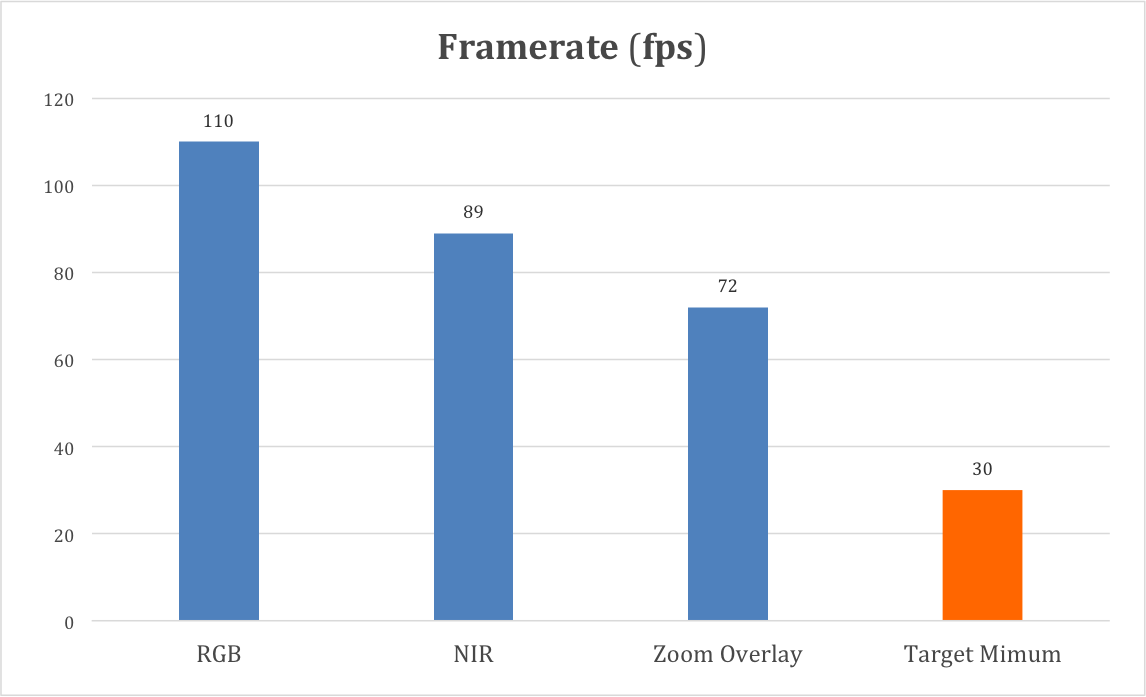
\includegraphics[width=0.7\textwidth]{images/framerate.png}
\caption{Frame Rate Measurements}
\end{figure}

\begin{figure}[H]
\centering
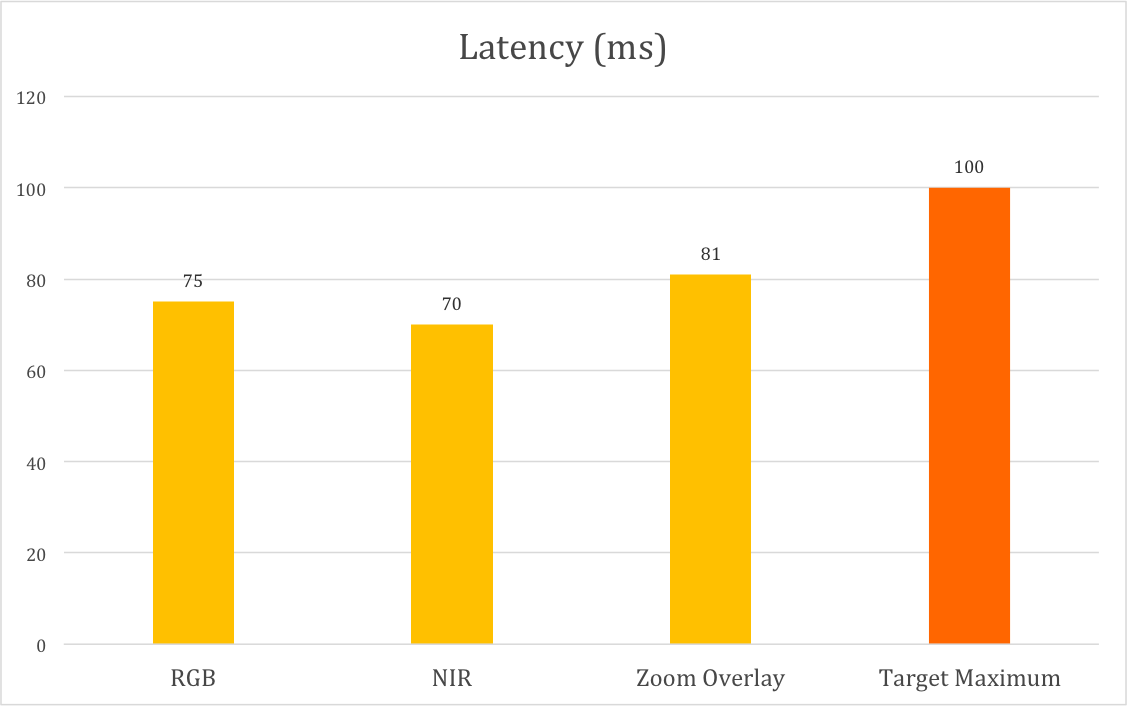
\includegraphics[width=0.7\textwidth]{images/latency.png}
\caption{Latency Measurements for RGB Camera Pipeline}
\end{figure}

\par
After having poor initial results using OpenCV, we decided to completely implement our own vision processing platform that utilizes GPU optimized video processing with the CUDA library. Our new vision platform takes advantage of the shared memory of the CPU and GPU on the Jetson by using a CUDA feature called Zero Copy. This allows us to create buffers that are shared directly between the CPU and GPU, without having to copy the image every time it is used. We integrated this functionality directly into our camera input system by allocating a shared memory buffer and setting up PointGrey's colorspace conversion to output directly into this buffer. Once the image is in GPU memory, we then are able to perform extremely fast operations on it using the GPU. Finally, we map the CUDA buffer to an OpenGL texture, which is then drawn to the screen.
\par
Using CUDA for our image processing system allowed us to meet high performance metrics, as we were able to add new filters with virtually no effect on frame rate or latency. Even a seemingly intensive edge detection algorithm causes a reduction of less than 1 frame per second. However, we were still limited on our frame rate by the input module. The 35-40fps we were acquiring was acceptable for our requirements, but our cameras are capable of much greater frame rates: up to 166fps at 1080p. By inserting timing measurements into each step in the input module, we were able to determine that the main cause of slowdown is the PointGrey colorspace conversion, which can take up to 30ms to complete depending on the camera. This initially limited us to lower frame rates, but by threading the input module we were able to perform multiple conversions at the same time. This enabled us to achieve much higher frame rates, up to 110fps with a single camera. Our latency increased slightly to about 40ms, but this is still within our 100ms acceptable range.
\par
Our new CUDA-based system is extremely fast, and enables us to work on more advanced image processing algorithms. Our current software includes multiple combination filters which blend two images together by averaging their color values, as well as a edge detection filter that was provided by NVIDIA in their CUDA sample code. Even with three camera inputs, two combination filters, and an edge detection filter, we still achieve roughly 85 frames per second without even coming close to our latency requirement. The image in figure 8 below displays this frame rate and the high quality of the image achieved in the output video stream from our Jetson TX1 and USB 3.0 PointGrey camera.
\par
Since the beta release, we have focused on decreasing our latency and increasing throughput. Our new method of measuring latency includes both the camera hardware and the monitor latency. This means that our new measurements are much higher than the original results. Our original CUDA based module has under 25ms latency, however the video feed is only monochrome. With our new RGB conversion algorithm, the output was slightly over the 100ms limit. By making some improvements that were suggested by our sponsors, we were able to bring the latency down to just about 75ms with our frame rate is still averaging around 90fps, which is triple the requirement. Figure 9 shows our most current latency measurements for the different features along with the corresponding frame rate speed shown in figure 8. Additionally, the latency and frame rate are very minimally affected by having multiple cameras compared to one, so even with our multi-camera system the latency is still low.
\par
After our beta release, we also worked on eliminating a number of bugs. We had been having random segfaults and occasional system crashes on program exit. We figured out that the segmentation faults were because of the software trying to use the camera before it had been fully initialized, so we added in a delay that allows the camera to boot up before capturing video from it. The system crashes were because of memory leaks in the CUDA part of the application, which would build up after running the program multiple times. Our new software properly cleans up all allocated GPU buffers and also resets the hardware's state upon exit.\\

\subsection{Installation and Execution}
This software is designed to be a proof of concept that demonstrates the computing power of the NVIDIA Jetson TX1. It is not meant to be installed on other hardware, as it requires the use of the GPU present in the Jetson, and is specifically optimized to use the Jetson's CPU/GPU shared memory that is not present on other devices. There are a number of example programs created using various filters and elements of the HawkEye system. They are run simply by executing them on the console.
\par
This software is designed specifically for the NVIDIA Jetson TX1 and for use with Point Grey USB 3.0 Cameras. It can be recompiled for other systems with CUDA-enabled GPUs however this has not been tested.

\subsection {Example Controls}
The example program we used at Expo has several controls.\\

Camera Views:
\begin{description}[leftmargin=2cm,labelindent=2cm]
	\item[{[1]}] RGB Camera
	\item[{[2]}] NIR Camera
	\item[{[3]}] Zoom Camera\\
\end{description}

Filters:
\begin{itemize}[leftmargin=2cm,labelindent=2cm]

\item RGB and Zoom Camera Views:
\begin{description}[leftmargin=2cm,labelindent=2cm]
	\item[{[F]}] Enable edge detection
	\item[{[G]}] Disable edge detection
	\item[{[H]}] Decrease edge detection threshold (more edges)
	\item[{[J]}] Increase edge detection threshold
	\item[{[\{]}] Zoom out
	\item[{[\}]}] Zoom in
\end{description}

\item RGB Only:
\begin{description}[leftmargin=2cm,labelindent=2cm]
	\item[{[Z]}] Enable zoom overlay
	\item[{[X]}]  Disable zoom overlay
\end{description}

\item IR Only:
\begin{description}[leftmargin=2cm,labelindent=2cm]
	\item[{[A]}] Decrease IR Threshold (brighter image)
	\item[{[S]}]  Increase IR Threshold (see only bright lights)\\
\end{description}

\end{itemize}

Quit Programs:
\begin{description}[leftmargin=2cm,labelindent=2cm]
	\item[{[Q]}]  Quit\\
\end{description}

